\subsection{Single-process system call latencies}
\label{eval:perf:syscall}


In order to understand the overheads of individual system calls,
Table~\ref{tab:graphene:lmbench} lists 
a representative sample of 
tests from the
\lmbench{} suite, version 2.5~\cite{McVoy:lmbench}.
Each row reports a mean and 95\% confidence interval;
we use the default number of iterations for each test case.
%We have added code to \lmbench{} to also calculate 95\% confidence intervals 
%within a run~\footnote{The lmbench authors deliberately exclude variation statistics
%because most methods assume a known distribution, generally a normal distribution---an 
%assumption which is often not the case for a computer microbenchmark~\cite{staelin05lmbench}.
%Though confidence intervals should be taken with a grain of salt, 
%we include them because they clearly indicate that these experiments have very low variance. In 
%a few cases of minor performance improvement, one can assess the impact of noise.}.
To measure the marginal cost of the reference monitor, we report numbers with and without 
the reference monitor.

%The performance of \graphene{} relative to Linux varies
%based on the system call.  
In general, calls that can be serviced inside the library are faster than native,
whereas calls that require translation to a native call incur overheads typically under 100\%.
For instance, 
the self-signaling test (sig overhead)
just calls the signal handler as a function,
which is almost twice as fast
as the Linux kernel implementation.  

\begin{table}[t!b!]
\footnotesize
\centering
\begin{tabular}{|l|rr|rrr|rrr|}
\hline
{\bf Test } & \multicolumn{2}{c|}{{\bf Linux}} & \multicolumn{3}{c|}{{\bf \graphene{}
}} & \multicolumn{3}{c|}{{\bf \graphene{} + SC + RM}} \\
&
\usec{} & +/- & 
\usec{} & +/- & \%O &
\usec{} & +/- & \%O \\

\hline

syscall        &  0.045 & .000 &  0.014 & .000 & -68.9 &    0.014 & .000 & -68.9   \\\hline
read           &  0.115 & .000 &  0.118 & .000 &   2.6 &    0.118 & .000 &   2.6   \\\hline
write          &  0.115 & .000 &  0.115 & .000 &   0.0 &    0.115 & .000 &   0.0   \\\hline
stat           &  0.332 & .000 &  1.154 & .000 & 247.6 &    1.161 & .000 & 249.7   \\\hline
fstat          &  0.107 & .000 &  0.189 & .000 &  76.6 &    0.189 & .003 &  76.6   \\\hline
open/close     &  0.880 & .003 &  2.552 & .005 & 190.0 &    2.816 & .002 & 330.0   \\\hline
select file    &  3.360 & .001 & 11.536 & .003 & 243.3 &   11.647 & .004 & 246.6   \\\hline
select tcp     & 10.590 & .002 & 11.679 & .002 &  10.3 &   12.050 & .000 &  13.8   \\\hline
sig install    &  0.126 & .000 &  0.126 & .000 &   0.0 &    0.126 & .000 &   0.0   \\\hline
sigusr1        &  0.951 & .000 &  0.184 & .000 & -80.7 &    0.188 & .000 & -80.2   \\\hline
sigsegv        &  0.263 & .000 &  1.467 & .000 & 457.8 &    1.681 & .000 & 539.2   \\\hline
\hline
TCP            &  8.354 & .001 &  9.121 & .002 &   1.8 &    9.699 & .002 &  16.1   \\\hline
UDP            &  7.222 & .002 &  9.450 & .002 &  30.8 &    9.995 & .001 &  38.4   \\\hline
AF\_UNIX       &  4.937 & .011 &  5.024 & .001 &   1.8 &    6.155 & .010 &  24.7   \\\hline
\hline
fork+exit      &  66.86 & 0.09 &   380.47 & 3.55 & 469 &   442.83 & 1.39 &   562   \\\hline
fork+fork+exit & 148.32 & 0.55 &   778.00 & 6.87 & 424 &   915.67 & 3.35 &   517   \\\hline
vfork+exec     & 141.53 & 0.18 &   487.67 & 5.05 & 245 &   547.30 & 5.22 &   286   \\\hline
fork+exec      & 194.93 & 0.20 &   810.00 & 3.27 & 315 &   878.50 & 1.89 &   350   \\\hline
fork+fork+exec & 266.89 & 0.36 & 1,200.60 & 5.20 & 349 & 1,387.75 & 6.21 &   420   \\\hline
fork+sh        & 499.64 & 0.67 & 1,726.75 & 6.14 & 245 & 1,912.00 & 3.83 &   283   \\\hline
%\hline
%UDP lat.&7.26&0.0&10.35&0.1&43&11.63&0.1&60 \\\hline
%TCP lat.&8.70&0.0&9.84&0.1&13&11.48&0.1&32 \\\hline
%\hline
%%%  \bf{Test} & K/s & +/- & K/s & +/- & \%O & K/s & +/- & \%O \\\hline
%%% %% \bf{Test} & \bf{K/s} & \bf{+/-} & \bf{K/s} & \bf{+/-} & \bf{\%O} & \bf{K/s} & \bf{+/-} & \bf{\%O} \\\hline
%%% 0K creat & 174 & 0.9 & 72 & 0.1 & 143 & 77 & 0.2 & 125 \\\hline
%%% 0K del & 232 & 1.2 & 130 & 0.5 & 79 & 117 & 0.2 & 98 \\\hline
%%% 4K creat & 120 & 0.1  & 33 & 0.0 & 265 & 31 & 0.0 & 284 \\\hline
%%% 4K del & 184 & 1.3  & 112 & 0.1 & 64 & 104 & 0.2 & 78 \\\hline
%%% 10K creat & 83 & 0.1  & 28 & 0.0 & 195 & 27 & 0.0 & 204 \\\hline
%%% 10K del & 149 & 0.3  & 94 & 0.1 & 58 & 88 & 0.2 & 69 \\\hline
\end{tabular}
\caption[\lmbench{} benchmarking results in Linux, KVM and \graphene{}]
{\lmbench{} comparison among (1) native Linux processes, (2) \graphene{} \picoprocs{} on Linux host, both without and with the SECCOMP filter ({\bf +SC}) and reference monitor ({\bf +RM}), and (3) \graphene{} in SGX enclaves.
Execution time is in microseconds, and lower is better. 
%The file system is measured in thousands operations per second, and higher is better.
Overheads are relative to Linux; negative overheads indicate improved performance.} 
\label{tab:graphene:lmbench}
\end{table}


The most expensive system calls occur when {\tt libLinux} inadvertently duplicates work
with the host kernel.  
For instance, many of the file path and handle management calls duplicate some of the effort of the host file system,
leading to a 1--3\x{} slower implementation than native.
As the worst example,
{\tt fork+exit} is 5.9\x{} slower than Linux.
Profiling indicates that about one sixth of this overhead is in process creation, which 
takes additional work to create a clean \picoproc{} on Linux; we expect this overhead could be reduced
with a kernel-level implementation of the process creation ABI, rather than emulating this behavior on {\tt clone}.
Another half of the overhead comes from the
{\tt libLinux} checkpointing code (commensurate with the data in Table~\ref{tab:graphene:lmbench}), which 
includes a substantial amount of serialization effort which might be reduced by checkpointing the data structures in place.
A more competitive {\tt fork} will require host support and additional {\tt libLinux} tuning.
%Thus, we think a competitive {\tt fork} implementation will require both a more suitable host kernel
%and more tuning in the {\tt libLinux} code. 
%\fixmewkj{explain why TCP faster than UDP?}



In this section we evaluate a few system operations that are heavily impacted by the \graphenesgx{} design.
%To shield dynamic loading and process creation,
%\graphenesgx{} uses computationally-expensive cryptographic techniques \fixmedp{more specific?} to verify enclave inputs.
% under the circumstance that the host OS cannot be trusted.
%As a trade-off to the security, the performance will be affected
%by additional cryptographic computation.
We measure the \syscall{open}, \syscall{read}, and \syscall{fork} system calls
using LMbench 2.5~\cite{McVoy:lmbench}.
A primary source of the overheads on these system calls is the cost of shielding applications, with run-time checks on the inputs.
Cryptographic techniques are used to: (1) validate the file against the secure hash, at \syscall{open}, (2) check the file chunks against the Merkle tree, at \syscall{read}, and (3) establish a TLS connection over inter-enclave RPC, at \syscall{fork}.
%opening a integrity-sensitive file for the first time, 
% or using cryptographic techniques, such as secure hashing, to verify the inputs.
% microbenchmarking specific system calls: 
% system calls,
%with different application settings.
%The microbenchmark is part of the LMBench 2.5 test suite
%\fixmedp{maybe merge this in the above paragraph, which feels a little coy}
%For instance, in order to shield dynamic loading, \graphenesgx{} checks each binary file against the secure hashes in the manifest,
%when the file is opened for the first time---after the whole file is copied into the enclave.
%\fixmedp{This happens after they are copied into enclave, memory right?}
%The verification happens when opening the file for the first time (often by the 
%After \graphenesgx{} validates the file, we generate a series of hashes of the file in chunks, as a merkle tree.
%to prevent verifying the whole file again when later randomly reading a part of the file.
%\fixmedp{So is this for the case when a file is swapped out?  I'm confused here - some details are missing}
%The latency of opening and reading an authenticated file in \graphenesgx{} is dominated by SHA256 and SHA512 calculation.
The remaining overheads contribute to exiting the enclave for host system calls, and bringing memory into the EPC (enclave page cache) or decrypting 
memory on a last-level cache miss. %and later the cache where the memory is decrypted by the CPU.


Figure~\ref{fig:syscall}(a)
shows the overhead for authenticating files in \syscall{open}.
\fixme{change overhead to latency}
Depending on the file size, the latency of \syscall{open} on \graphenesgx{} is 383$\mu$s (64KB file) to 21ms (4MB file), whereas on Linux, the latency is constant at 0.85$\mu$s.
We note that this is where enclaves are at a disadvantage, as \syscall{open} 
normally does not need to read file content; whereas here \graphenesgx{} uses \syscall{open}
as a point at which to validate file content.
For a subsequent \syscall{open}, when the Merkle tree is already generated, the overhead of simply exiting enclave for \syscall{open}, and searching the file list in the manifest, is about 9$\times$.
%\fixmedp{why?}


One might be able to optimize further for cases where only part of a file is accessed
with incremental hashing.  However, in the common case where nearly all of the file is accessed,
these costs are difficult to avoid when host file system is untrusted.
Another opportunity 
is to create the Merkle tree offline, when the manifest is created.
%\fixmedp{I think the second idea has legs...}


%This is an inevitable cost, because normal \funcname{open} on trusted OSes
%need not to access file content.
%After verifying the file, \graphenesgx{} buffers the chunk hash values, to skip whole-file verification when the file is reopened.

Figure~\ref{fig:syscall}(b)
shows the overhead for authenticating files in \syscall{read}, which 
is lower than \syscall{open}.
Since the whole file has been verified at \syscall{open}, the sequential \syscall{read} only verifies the chunks of files it is reading from untrusted memory.
%Reads from data cached in enclave memory are cheaper.  %\fixmedp{right? can we say how much cheaper?  Maybe add separate bars for both cases?}
% Therefore, \syscall{read} is actually much cheaper than \syscall{open}.
Depending on the size of blocks being read, the latency on \graphenesgx{} is 0.5$\mu$s (64-byte \syscall{read}) to 16.9$\mu$s (4KB \syscall{read}). The latency of \syscall{read} on Linux is \roughly{}0.1$\mu$s for any block size below 4KB.
If the file is not authenticated,
\graphenesgx{} only copies the file contents into the buffer, and the overhead reduces to 48\% (64-byte \syscall{read}) to 83\% (4KB \syscall{read}).
\fixmedp{Consider doing larger buffers, say up to 64k or even 4 MB}

%\fixmedp{In the legend for 7b, unsecure should be insecure}


Figure~\ref{fig:syscall}(c) shows the overhead of forking a process.
As described in \ref{sec:sgx:shield-multiproc}, the latency of \syscall{fork} in \graphenesgx{} is affected by three factors:
creation of a new enclave, local attestation of the integrity, and duplicating the process state over an encrypted RPC stream.
Combining these factors, \syscall{fork} is one of the most expensive calls in \graphenesgx{}.
%, but at least it is supported natively on the current hardware.
The default enclave size is 256MB.
%which takes \roughly{}0.5s to create. 
Our evaluation shows that the latency of forking a process is around 0.8s (16MB process) to 2.7s (128MB process), but can be more expensive if the parent process uses more memory.
The trend matches the performance of \graphene{} without the bulk IPC optimization.
\fixmedp{If you want, some thoughts on how this might be improved in the future would be nice...  One good suggestion is recycling enclaves, or pre-forking so measurements can be done in parallel}
%Due to the overhead on \funcname{fork}, \graphenesgx{} is not suitable for fork-intensive workloads like Bash scripts
%if performance is critical.

\fixme{talk about a limitation of improving fork. check this.}
One way to further optimize \syscall{fork} is to reduce or avoid enclave creation time; one can potentially pre-launch a child enclave, and then migrate the process contents later when \syscall{fork} is called.
There might be another opportunity to improve the latency of process migration,
if copy-on-write sharing of enclave pages can be supported in future generations of SGX.
%Unfortunately, sending the process contents is difficult to avoid in \syscall{fork},
%as SGX disallows sharing enclave memory between multiple enclaves.

%\fixmedp{I assume 5.4 isn't done yet}


%Adding more detail of KVM environment
%Unless otherwise noted, \graphenesgx{} measurements include the Phosphor instrumentation.





\begin{figure*}[t!]
\centering

\begin{minipage}{.45\textwidth}
\centering
\footnotesize
\vspace{6pt}
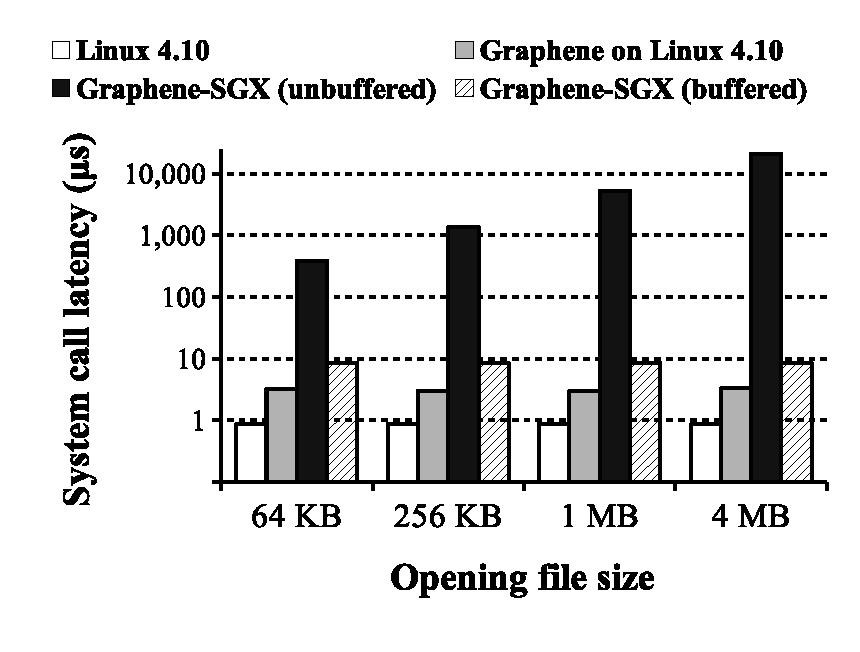
\includegraphics[width=\linewidth]{sgx/open-latency}\\
\vspace{3pt}
{\bf (a) Open a file}
\vspace{6pt}
\end{minipage}
\begin{minipage}{.45\textwidth}
\centering
\footnotesize
\vspace{6pt}
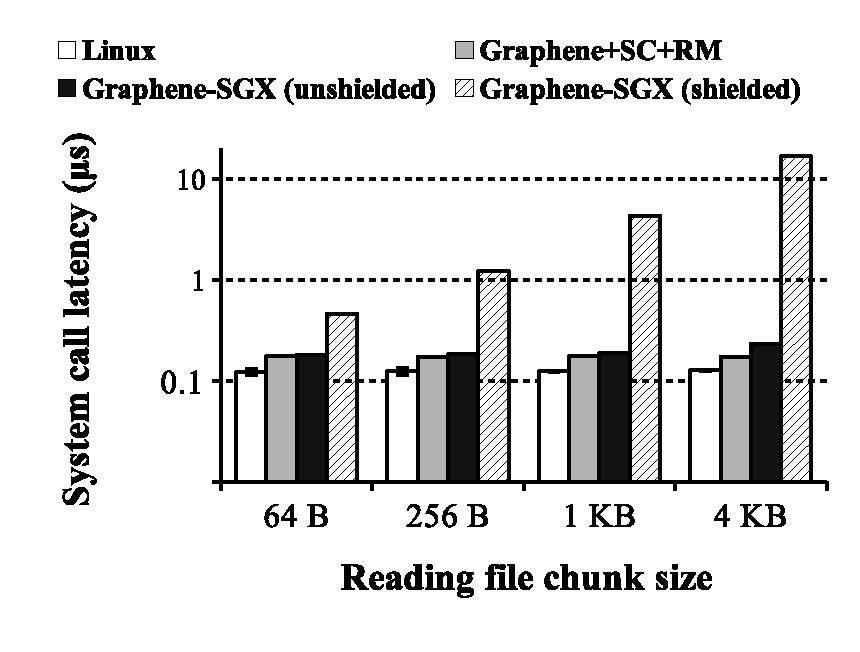
\includegraphics[width=\linewidth]{sgx/read-latency}\\
\vspace{3pt}
{\bf (b) Read a file}
\vspace{6pt}
\end{minipage}
\begin{minipage}{.45\textwidth}
\centering
\footnotesize
\vspace{6pt}
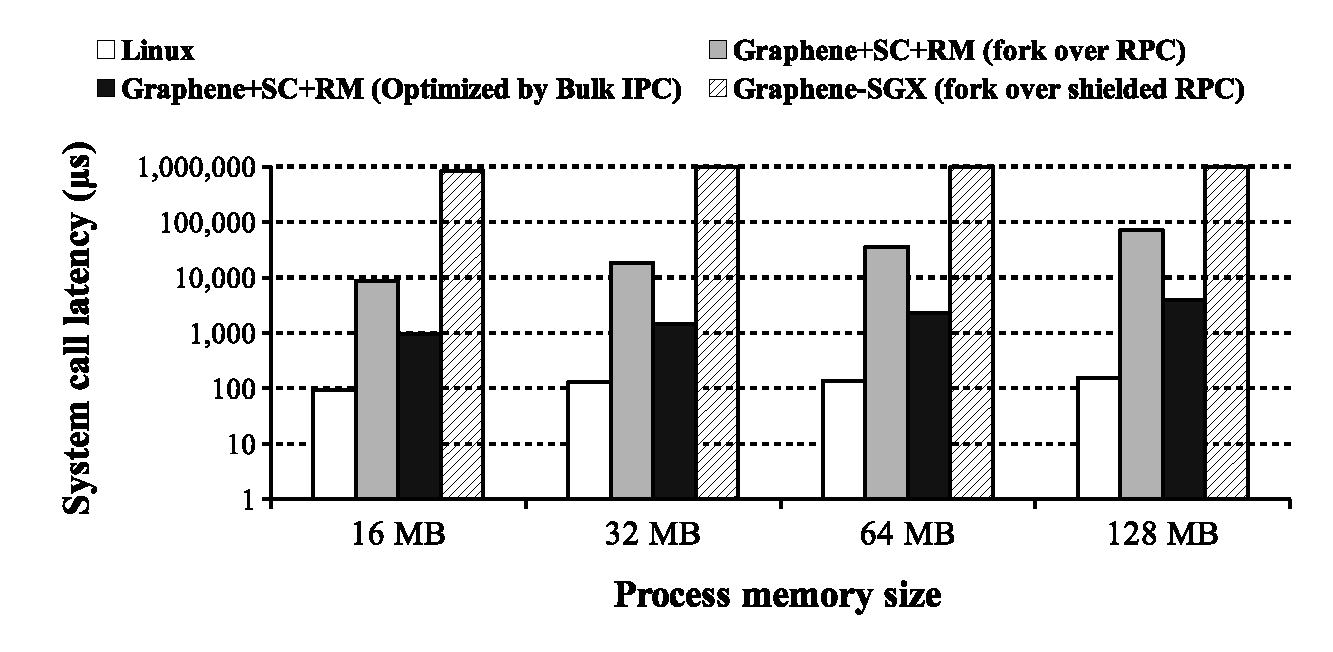
\includegraphics[width=\linewidth]{sgx/fork-latency}\\
\vspace{3pt}
{\bf (c) Fork a process}
\vspace{6pt}
\end{minipage}

\caption{Latency of some expensive system calls in \graphenesgx{}, including opening and reading a secured (authenticated) file, and forking a new process. The results are compared with native Linux and \graphene{}.}
\label{fig:syscall}
\end{figure*}

